To illustrate our stateful filtering process, we propose the following simple
example.
An electrical disconnector $D$ separates three electrical networks such as
networks 2 and 3 are connected to the same input of $D$.
As we told in Section~\ref{sec:intro}, a disconnector cannot be manipulated while
current is passing to avoid the creation of an electric arc.
To ensure safety, three circuit breakers $B_1$, $B_2$ and $B_3$ are placed
between $D$ and each electrical network.
Figure~\ref{fig:example} describes this setup.

\begin{figure}[htb]
    \centering
    \resizebox{.5\textwidth}{!}{
        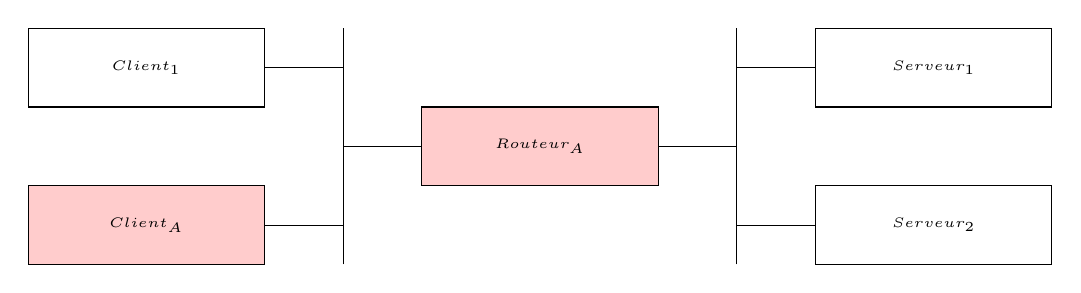
\begin{tikzpicture}[font=\tiny,
    arrow/.style={thick,<->,shorten >=2pt,shorten <=2pt,>=stealth},
]
    \draw[fill=red!20!white] (0,0) rectangle (3,1) node [pos=.5] {$Client_{A}$};
    \draw (0,2) rectangle (3,3) node [pos=.5] {$Client_1$};
    
    \draw[fill=red!20!white] (5,1) rectangle (8,2) node [pos=.5] {$Routeur_{A}$};

    \draw (10,0) rectangle (13,1) node [pos=.5] {$Serveur_{2}$};
    \draw (10,2) rectangle (13,3) node [pos=.5] {$Serveur_{1}$};
    
    \draw (3,.5) -- (4,.5); 
    \draw (3,2.5) -- (4,2.5); 
    \draw (4,1.5) -- (5,1.5);
    \draw (4,0) -- (4,3);

    \draw (9,.5) -- (10,.5); 
    \draw (9,2.5) -- (10,2.5); 
    \draw (8,1.5) -- (9,1.5);
    \draw (9,0) -- (9,3);
\end{tikzpicture}

    }
    \caption{Example infrastructure}
    \label{fig:example}
\end{figure}

Within a \modbus server, $D$, $B_1$, $B_2$ and $B_3$ can be represented as coil
(i.e.: read/write booleans) with opened state represented by {\em False}.
In this example, $D$ can be manipulated if and only if either $B_1$ if opened
or if both $B_2$ and $B_3$ are open.
Thus the configuration presented in Listing~\ref{lst:example} is enough to
describe this rule.
Note that in the rule definition, the AND operator has priority on the OR
operator.

\begin{lstlisting}[label=lst:example,caption=Example configuration]
Declare Server 1 Protocol Modbus Addr 10.0.0.1 Port 502
<@\vspace{-.8em}@>
Declare Variable 1 Server 1 Type Boolean Addr coils:0x1001 # <@{\color{Green} $B_1$}@>
Declare Variable 2 Server 1 Type Boolean Addr coils:0x1002 # <@{\color{Green} $B_2$}@>
Declare Variable 3 Server 1 Type Boolean Addr coils:0x1003 # <@{\color{Green} $B_3$}@>
Declare Variable 4 Server 1 Type Boolean Addr coils:0x1004 # <@{\color{Green} $D$}@>
<@\vspace{-.8em}@>
Declare Monitor 1 Variable 1 # Monitor on <@{\color{Green} $B_1$}@>
Declare Monitor 1 Variable 2 # Monitor on <@{\color{Green} $B_2$}@>
Declare Monitor 1 Variable 3 # Monitor on <@{\color{Green} $B_3$}@>
<@\vspace{-.8em}@>
Declare Rule Variable 4 Assert    \
    Equal(LocalVal[1], False) OR \
    Equal(LocalVal[2], False) AND Equal(LocalVal[3], False)
\end{lstlisting}

Thus, any sequence of message violating the rule will be blocked ensuring the
safety of the disconnector.
